\documentclass[
  a4paper,
  12pt,
  dvipdfmx
]{jsarticle}
\usepackage{titling}
\usepackage{amsmath,amssymb}
\usepackage{amsthm} %定理環境
\usepackage{bm}
\usepackage{url}
\usepackage[dvipdfmx]{graphicx, color}
\usepackage{ascmac}
\usepackage{enumerate} %箇条書き
\usepackage{enumitem}
\usepackage{mathtools}
\usepackage{amsfonts}
\usepackage{latexsym}
% \usepackage[all]{xy}
% \usepackage{ulem} %波線
\usepackage[normalem]{ulem}
% %\usepackage{eclbkbox}%四角枠 
\usepackage[titles]{tocloft}%体裁を整える
\usepackage{titlesec}%見出しの設定
\usepackage{float}%図の位置
\usepackage{mathrsfs}%花文字
\usepackage{tikz}
\usepackage[dvipdfmx]{hyperref}
\usepackage{pxjahyper} % (u)pLaTeXのときのみかく
\usepackage{docmute} %分割に必要 
\usepackage{tikz-cd} %可換図式
% \usepackage[margin=30truemm]{geometry}
% \usepackage{authblk}
\usepackage{appendix}
\usepackage{caption}
\usetikzlibrary{arrows.meta}
\usetikzlibrary{patterns}
\usetikzlibrary{spath3}
\usetikzlibrary{knots}
\usetikzlibrary{hobby}
\usetikzlibrary{external}

%自分用のコマンド
\providecommand{\cprime}{\hbox{$'$}} %bibtex用
\newcounter{questionCounter}% 新しいカウンターを定義
\newcommand{\Qbox}{\stepcounter{questionCounter}\fbox{\thequestionCounter}}
\newcommand{\RR}{\mathbb{R}}
\newcommand{\CC}{\mathbb{C}}
\newcommand{\engname}[1]{(\textbf{#1})}
\newcommand{\te}{\textrm{there exists\ }}
\newcommand{\st}{\ \textrm{such that}\ }
\newcommand{\mcal}[1]{\mathcal{#1}}
\newcommand{\fall}{\textrm{for all}\ }
\newcommand{\suml}[2]{\sum\limits_{#1}^{#2}}
\newcommand{\simpangle}[1]{\langle#1\rangle}
\newcommand{\ZZ}{\mathbb{Z}}
\newcommand{\NN}{\mathbb{N}}
\newcommand{\QQ}{\mathbb{Q}}
\newcommand{\ca}{\mathcal{A}}
\newcommand{\ck}{\mathcal{K}}
% 卒論
\setlength{\topmargin}{0truecm}
\newcommand{\TITLE}%
{タイトル未定}
\newcommand{\STNO}%
{2264246}
\newcommand{\NAME}%
{宮路 宙澄}%氏名
\newcommand{\ADVR}%
{野崎 雄太 准教授}
\newcommand{\DATE}%
{(2026年1月30日)}
\DeclareMathOperator{\Ker}{Ker}
\DeclareMathOperator{\rank}{rank}
\DeclareMathOperator{\gr}{gr} %graded
\DeclareMathOperator{\id}{id} %id
\DeclareMathOperator{\proj}{proj}

\let\Re\relax%実部虚部の更新
\DeclareMathOperator{\Re}{Re}
\let\Im\relax
\DeclareMathOperator{\Im}{Im}

\title{
  \centerline{\mbox{卒論(タイトル未定)}}
  % Jones 多項式と Vassiliev 不変量の導入と関係性\\
  \large 元論文: Homomorphic expansions for knotted trivalent graphs
}
\author{宮路 宙澄}
\date{\today}
\hypersetup{
  colorlinks=false,
  pdfborder={0 0 1},
  linkbordercolor={red},
}

\renewcommand{\theenumi}{\roman{enumi}}
\renewcommand{\labelenumi}{(\theenumi)}
\renewcommand{\theenumii}{\theenumi-\alph{enumii}}
\renewcommand{\labelenumii}{(\theenumii)}
\renewcommand{\theenumiii}{\theenumii-\roman{enumiii}}
\renewcommand{\labelenumiii}{(\theenumiii)}


\newcounter{mycounter} % 新しいカウンタを定義
\numberwithin{mycounter}{section} % mycounter を section と同期

\theoremstyle{definition}
\newtheorem{theorem}[mycounter]{Theorem}
\newtheorem{proposition}[mycounter]{Proposition}
\newtheorem{lemma}[mycounter]{Lemma}
\newtheorem{corollary}[mycounter]{Corollary}

\newtheorem{definition}[mycounter]{Definition}
\newtheorem{example}[mycounter]{Example}
\newtheorem{remark}[mycounter]{Remark}
\newtheorem{exercise}[mycounter]{Exercise}
\begin{document}
% \maketitle
\thispagestyle{empty}
\hfil 2025年度 横浜国立大学 理工学部 数理科学EP 卒業研究
\vskip3cm
{
  \Large
  \begin{center}
    \huge
    \textbf{\TITLE}
  \end{center}
  \vfill
  \hfil
  {
    \LARGE\textbf{\STNO\ \NAME}
  }
  \vskip10Q
  \hfil\textbf{指導教員:\ADVR }\hfil\textbf{\DATE}
}
\vfill
\hfill
\begin{tabular}{|p{6zw}|p{6zw}|} \hline\hskip.5zw 指導教員印 & \hskip1.5zw 受理印 \\
  \hline& \\
  [2cm] \hline 
\end{tabular}
\newpage
\begin{abstract}
  【保留】
  KTGsに対し a universal Vassiliev invariant が存在することは知られていた\cite{murakami1997topological,cheptea2007tqft,dancso2010kontsevich}.
  KTGsにおいて``edge unzip''という演算のみ準同型にならず,補正項が現れる.dotted Knotted Trivalent Graphs において$Z^{old}$が準同型となるように$Z$を2通りで構成することが目的.
\end{abstract}
\tableofcontents
\newpage

\section{Introduction}
結び目理論とは位相幾何学の分野の一つであり,物理学とも関係する分野である.その中でも,結び目同士が異なるかどうかを区別する際に手段として使われるものとして結び目の不変量というものがある.

% Knotted Trivalent Graphs(Knots や links を含む) のなす空間には良い構造がある.
% 次の4つの操作がある: orientation switch, edge delete, edge unzip, connected sum.
% KTGs は有限生成である\cite{thurston2002algebra}.
% %要確認
% KTGsはKnot genus(ザイフェルト曲面?)やribbon property(ribbon knot?自己交差あり)などの良い代数構造をもつため,それらを使うことが出来る\cite{bar898algebraic}.

% Knots の Kontsevich integral は universal Vassiliev invariant に拡張できる.
% その中でも unzip 以外が準同型になる.
% \begin{itemize}
%   \item unzip, delete, connected sum を``tree connected sums''と呼ばれるより一般の操作へ変える.
%   \item unzip が出来る edge を制限する.
% \end{itemize}
% 簡単に$Z^{old}$をdKTGsで準同型にすることができ,dKTGsはKTGsの良い性質をすべて保つことを示す.
% 有限生成やclose connection to Drinfel'd associators (知らん) など.
\section{Acknowledgements}
\newpage
\section{Preliminaries}
\subsection{KTGs and $Z^{old}$}

% \begin{definition}
%   \textbf{Trivalent graph}(3価グラフ)とは,各頂点が3つの辺をもつようなグラフをいう.
% \end{definition}

グラフにおいて,全ての辺は向きづけられているものとし,頂点は反時計回りに向きを与える.また,ループや円などの辺を許すこととする.

\begin{definition}
  \textbf{滑らかな曲面 (surface)}とはコンパクトで向き付け可能で第2可算公理\footnote{高々可算な開基を持つ.}を満たす境界付き2次元 $C^\infty$ 級多様体をいう.
\end{definition}

\begin{definition}
  単体複体 $Y$ の \textbf{spine} $X$ とは,$Y$ の部分複体 $X$ であって,$Y$ を $X$ へ潰すことができるものをいう.ここで\textbf{潰す (collapse)}とは,$k$-単体 $\Delta^{k}$ と $(k+1)$-単体 $\Delta^{k+1}$ の対を取り除いていく操作のことをいう.ただし,$\Delta^{k+1}$ はその境界上に $\Delta^{k}$ を持つような唯一の $(k+1)$-単体でなければならない.
\end{definition}

\begin{definition}
  グラフ $\Gamma$に対し \textbf{枠付きグラフ (framed graph)} $\mathbf{\Gamma}$とは,1次元単体複体 $\Gamma$ と, $\Gamma$ を滑らかな曲面 $\Sigma$ に spine となるように埋め込む写像 $\Gamma\hookrightarrow\Sigma$ の組 $(\Gamma, \Sigma)$ のことである.ここで,$\Gamma$ への埋め込みは各辺の内部において滑らかであるものとする.
  特に $\Gamma$ が3価グラフのとき,$\mathbf{\Gamma}$を\textbf{枠付き3価グラフ (framed trivalent graph)}という.
  % For a graph $\Gamma$, a \textbf{framed graph} $\mathbf{\Gamma}$ is a pair $(\Gamma, \Sigma)$ of 1-dimensional simplicial complex $\Gamma$ and an embedding $\Gamma\hookrightarrow\Sigma$ of $\Gamma$ into a surface $\Sigma$ as a spine. In particular, when $\Gamma$ is a trivalent graph, it is called a \textbf{framed trivalent graph}.
\end{definition}

2つの枠付きグラフ $\mathbf{\Gamma} = (\Gamma, \Sigma), \mathbf{\Gamma}' = (\Gamma', \Sigma')$ が同値であるとは,$\Sigma$ から $\Sigma'$ への向きを保つ $C^\infty$ 級微分同相写像 $h\colon \Sigma \to \Sigma'$ が存在し,$h(\Gamma) = \Gamma'$ となることをいう.このとき,$h$ はグラフ同型 $\Gamma\to\Gamma'$ を誘導し,各頂点において反時計周りの順序を保つ.以下では枠付きグラフはこの同値関係のもとで考える.また,枠付きグラフはこの同値関係のもとで一意に定まる.
% We regard two framed graphs $(\Gamma, \Sigma)$ and $(\Gamma, \Sigma')$ as equivalent if there exists an orientation-preserving diffeomorphism $h\colon \Sigma \to \Sigma'$ such that $h|_{\Gamma} = \id_{\Gamma}$. We consider framed graphs up to this equivalence. Under a fixed cyclic ordering of edges at each vertex, the framed graph is uniquely determined up to this equivalence.

\begin{definition}
  枠付き3価グラフ $\mathbf{\Gamma} = (\Gamma, \Sigma)$ に対し,\textbf{knotted trivalent graph (KTG)} $\gamma$ とは,枠付きグラフ $\mathbf{\Gamma} = (\Gamma, \Sigma)$ と滑らかな埋め込み写像 $g\colon \Sigma \hookrightarrow \RR^3$ の組 $(\Gamma, \Sigma, g)$ のことである.また,KTG $\gamma = (\Gamma, \Sigma, g)$ の\textbf{骨格 (skeleton)}とは,$\Gamma$ のことである.
  % For a framed trivalent graph $\mathbf{\Gamma}=(\Gamma,\Sigma)$, a \textbf{knotted trivalent graph (KTG)} $\gamma$ is a triple $(\Gamma, \Sigma, g)$ consisting of the framed graph $\Gamma$ and an embedding $g\colon \Sigma\hookrightarrow\RR^3$. The \textbf{skeleton} of a KTG $\gamma$ is the trivalent graph $\Gamma$ behind it.
  \begin{figure}[H]
    \centering
    \raisebox{-0.4\height}{\includegraphics[scale=0.3]{inkscape/trivalentgraph.pdf}}
    $\leadsto$
    \raisebox{-0.4\height}{\includegraphics[scale=0.23]{inkscape/framedtrivalentgraph.pdf}}
    \caption{枠付き3価グラフの例}
  \end{figure}
  \begin{figure}[H]
    \centering
    \raisebox{-0.4\height}{\includegraphics[scale=0.3]{inkscape/exKTG.pdf}}
    \caption{Knotted trivalent graph の例}
    \label{fig:exKTG}
  \end{figure}
\end{definition}

以降の図では,knotted trivalent graph を書く際には黒板上の枠付けを用い,曲面を省略し骨格のみを描く.

\begin{definition}
  枠付きグラフを $\mathbf{\Gamma} = (\Gamma, \Sigma)$ とする.このとき,2つの knotted trivalent graphs $\gamma_1 = (\Gamma, \Sigma, g), \gamma_2 = (\Gamma, \Sigma, h)$ が\textbf{枠付きイソトピック (framed isotopic)} であるとは,滑らかな埋め込み
  \[
    \Phi \colon \Sigma \times I \to \RR^3 \times I\quad (I=[0,1])
  \]
  が存在し,次の条件を満たすことをいう:
  \begin{enumerate}
    \item 任意の $x \in \Sigma$ と $t \in I$ に対し,$\Phi(x,t) = (\varphi_t(x), t)$ となる滑らかな埋め込み $\varphi_t \colon \Sigma \hookrightarrow \RR^3$ が存在する,
    \item $\varphi_0 = g$ かつ $\varphi_1 = h$ である.
  \end{enumerate}
  % Two knotted trivalent graphs $\gamma_1=(\Gamma, \Sigma, g)$ and $\gamma_2=(\Gamma, \Sigma, h)$ are said to be \textbf{framed isotopic} if there exists a smooth embedding
  % \[
  %   \Phi \colon \Sigma \times I \to \RR^3 \times I\quad (I=[0,1])
  % \]
  % satisfying the following conditions:
  % \begin{enumerate}
  %   \item $\Phi$ is level-preserving, that is, for any $x \in \Sigma$ and $t \in I$, $\Phi(x,t) = (\varphi_t(x), t)$ for a smooth embedding $\varphi_t \colon \Sigma \hookrightarrow \RR^3$,
  %   \item The restriction $\Phi|_{\Gamma\times I}$ is an identity,
  %   \item $\varphi_0 = g$ and $\varphi_1 = h$.
  % \end{enumerate}
\end{definition}
以下では knotted trivalent graphs を枠付きイソトピックで同一視する.
ここで,骨格が $\Gamma$ である全ての knotted trivalent graphs の線形結合からなる $\QQ$ 上のベクトル空間を次のように表す:
% We identify KTGs whose are framed isotopic. For a trivalent graph $\Gamma$, we denote the vector space over $\QQ$ generated by all linear combinations of KTGs with skeleton $\Gamma$ by
\[
  \mathcal{K}(\Gamma)\coloneqq\left\{\sum_{i=1}^m a_i \gamma_i\,\middle|\, m\in\ZZ_{> 0}, a_i\in \QQ, \gamma_i\text{: }\Gamma \text{ を骨格とする KTG.}\right\}.
\]
\begin{definition}
  3価グラフ $\Gamma$ に対し,$\Gamma$ を台とする\textbf{次数 n のコード図 (chord diagram of order n)}とは,$\Gamma$と,$\Gamma$ 上の相異なる $2n$ 個の点の組をいい,各2点の組を結ぶ線を\textbf{コード (chord)}という.ここで,コードは骨格とは区別された点線として視覚化される.
  % 3価グラフ $\Gamma$ に対し,\textbf{コード図 (chord diagram)} $D$ とは,$\Gamma$ と,$\Gamma$ 上に1価頂点を持つ頂点向き付きの1,3価グラフからなる組であり,そのグラフは円に同相な連結成分を持たないものである.
  % For a graph $\Gamma$, a \textbf{chord diagram} $D$ with support $\Gamma$ is $\Gamma$ together with an vertex-oriented uni-trivalent graph whose univalent vertices are on $\Gamma$; and the graph does not have any connected component homeomorphic to a circle. We call the uni-trivalent graph the chord graph of the diagram.
\end{definition}

\begin{proposition}
  2つの knotted trivalent graphs が枠付きイソトピックであることと,それらのコード図が有限回の Reidemeister 変形 $R1', R2, R3, R4$ で移り合うことは同値である.
  % Two KTGs are framed isotopic if and only if their graph diagrams are related by a finite sequence of Reidemeister moves $R1', R2, R3$ and $R4$.
  \begin{center}
    $R1'$:\hspace{2mm}
    \raisebox{-0.45\height}{\includegraphics[scale=0.5]{inkscape/FramedReideMoves/fR1_0.pdf}} \hspace{3mm}$\longleftrightarrow$ \hspace{3mm}
    \raisebox{-0.45\height}{\includegraphics[scale=0.5]{inkscape/FramedReideMoves/fR1_1.pdf}} \hspace{3mm}$\longleftrightarrow$\hspace{3mm}
    \raisebox{-0.45\height}{\includegraphics[scale=0.5]{inkscape/FramedReideMoves/fR1_2.pdf}}
    
    \vspace{3mm}
    $R2$:\hspace{2mm}
    \raisebox{-0.45\height}{\includegraphics[scale=0.5]{inkscape/FramedReideMoves/fR2_0.pdf}} \hspace{3mm}$\longleftrightarrow$ \hspace{3mm}
    \raisebox{-0.45\height}{\includegraphics[scale=0.5]{inkscape/FramedReideMoves/fR2_1.pdf}} \hspace{3mm}$\longleftrightarrow$\hspace{3mm}
    \raisebox{-0.45\height}{\includegraphics[scale=0.5]{inkscape/FramedReideMoves/fR2_2.pdf}}
    
    \vspace{3mm}
    $R3$:\hspace{2mm}
    \raisebox{-0.45\height}{\includegraphics[scale=0.5]{inkscape/FramedReideMoves/fR3_0.pdf}} \hspace{3mm}$\longleftrightarrow$ \hspace{3mm}
    \raisebox{-0.45\height}{\includegraphics[scale=0.5]{inkscape/FramedReideMoves/fR3_1.pdf}}

    \vspace{3mm}
    $R4a$:\hspace{2mm}
    \raisebox{-0.45\height}{\includegraphics[scale=0.5]{inkscape/FramedReideMoves/fR4a_0.pdf}} \hspace{3mm}$\longleftrightarrow$ \hspace{3mm}
    \raisebox{-0.45\height}{\includegraphics[scale=0.5]{inkscape/FramedReideMoves/fR4a_1.pdf}}
    \vspace{3mm}
    \noindent
    \begin{minipage}{\linewidth}
      \centering
      $R4b$:\hspace{2mm}
      \raisebox{-0.45\height}{\includegraphics[scale=0.5]{inkscape/FramedReideMoves/fR4b_0.pdf}} \hspace{3mm}$\longleftrightarrow$ \hspace{3mm}
      \raisebox{-0.45\height}{\includegraphics[scale=0.5]{inkscape/FramedReideMoves/fR4b_1.pdf}}
      \captionof{figure}{Knotted trivalent graphs における Reidemeister 変形}
      \label{fig:ReidemeisterKTG}
    \end{minipage}
  \end{center}
\end{proposition}
ここでは証明を省略する.詳細は\cite[Theorem~1.4]{murakami1997topological}を参照されたい.空間グラフに対して定義された拡張 Reidemeister 変形\cite{yamada1987invariant}に関して不変であることを示せば十分である.ここでは黒板上の枠付けを考えているため,頂点周りの辺の順序を変える変形は考慮しなくてよいことに注意されたい.\\
% We omit the proof here. For details, please refer to \cite[Theorem~1.4]{murakami1997topological}. It is sufficient to show the invariance under extended Reidemeister moves for spatial graphs defined in \cite{yamada1987invariant}. Note that we do not need the move in \cite{yamada1987invariant} which changes the order of edges around a vertex, since we consider framed graphs with the blackboard framing.\\
{\color{red}ここにつなぎの文が欲しい}\\
KTGs における演算を4つ定義する:
\begin{definition}
  $\Gamma$ を3価グラフ,$e$ を $\Gamma$ の辺とする.$e$ の向きを反転させることによって得られる3価グラフを $S_e(\Gamma)$ と表す.また,KTG $\gamma\in\mathcal{K}(\Gamma)$ に対し,辺 $e$ の\textbf{switch the orientation}を,$e$の向きを反転させることによって定義し,$S_e$ と表す.
  % Let $\Gamma$ be a trivalent graph and let $e$ be an edge of $\Gamma$.
  % We denote by $S_e(\Gamma)$ the graph obtained from $\Gamma$ by reversing the orientation of the edge $e$.
  % For a knotted trivalent graph $\gamma \in \mathcal{K}(\Gamma)$, the operation of \textbf{switch the orientation} of $e$ is defined by reversing its orientation, and is denoted by $S_e$.
  \[
    S_e \colon \mathcal{K}(\Gamma) \to \mathcal{K}(S_e(\Gamma)) \,;\, \gamma \mapsto S_e(\gamma)
  \]
  \begin{figure}[H]
  \centering
  \raisebox{-0.45\height}{\includegraphics{inkscape/switch.pdf}}
  \end{figure}
\end{definition}

\begin{definition}
  $\Gamma$ を3価グラフ,$e$ を $\Gamma$ の辺とする.$e$ を取り除き,さらにその両端に生じる2価頂点を取り除き1本の辺にすることによって得られるグラフを $d_e(\Gamma)$ と表す.このとき,$e$ の両端で $e$ に接続する2つの辺の向きが一致していることが必要である.また,KTG $\gamma\in \mathcal{K}(\Gamma)$ に対し,辺 $e$ の\textbf{delete}を同様に定義し,$d_e$ と表す.
  % Let $\Gamma$ be a trivalent graph and let $e$ be an edge of $\Gamma$. We denote by $d_e(\Gamma)$ the graph obtained from $\Gamma$ by removing $e$ and two vertices at the ends of $e$ and smoothing the two resulting bivalent vertices into single edges. To do this, it is required that the orientations of the two edges connecting to $e$ at either end match.
  % For a knotted trivalent graph $\gamma\in \mathcal{K}(\Gamma)$, the operation of \textbf{delete} of $e$ is defined in the same way, and is denoted by $d_e$.
  \[d_e\colon \mathcal{K}(\Gamma)\to\mathcal{K}(d_e(\Gamma))\,;\,\gamma\mapsto d_e(\gamma)\]
  \begin{figure}[H]
  \centering
  \raisebox{-0.45\height}{\includegraphics{inkscape/delete.pdf}}
  \end{figure}
\end{definition}

\begin{definition}
  $\Gamma$ を3価グラフ,$e$ を $\Gamma$ の辺とする.$e$ を十分近い2つの辺に置き換え,さらに両端の頂点を取り除くことによって得られるグラフを $u_e(\Gamma)$ と表す.このとき,$e$ の始点に接続する2つの辺は両方とも $e$ に入る向きであり,終点に接続する2つの辺は両方とも $e$ から出る向きでなければならない.また,KTG $\gamma\in\mathcal{K}(\Gamma)$ に対し,辺 $e$ の\textbf{unzip}を同様に定義し,$u_e$ と表す.
  % Let $\Gamma$ be a trivalent graph and let $e$ be an edge of $\Gamma$. We denote by $u_e(\Gamma)$ the graph obtained from $\Gamma$ by replacing $e$ with two edges that are ``very close to each other'', and the two vertices at the ends of $e$ will disappear. Again the edges at the vertex where $e$ begins have to both be incoming, while the edges at the vertex where $e$ ends must both be outgoing.
  % For a knotted trivalent graph $\gamma\in\mathcal{K}(\Gamma)$, the operation of \textbf{unzip} of $e$ is defined in the same way, and is denoted by $u_e$.
  \[u_e\colon \mathcal{K}(\Gamma)\to\mathcal{K}(u_e(\Gamma))\,;\,\gamma\mapsto u_e(\gamma)\]
  {\Large \color{red} 元の論文には$u_e(\Gamma)$とあるが,単なるグラフ$\Gamma$に対しては2つに分割する方法が一意に定まらないため,枠付きグラフ$\mathbf{\Gamma}$に対して定義する(これではwell-defにできる)べきではないか?その場合,$\mathcal{K}(\Gamma)$等の定義全てを$\mathcal{K}(\mathbf{\Gamma})$に変更する必要がある.}
  \begin{figure}[H]
  \centering
  \raisebox{-0.45\height}{\includegraphics{inkscape/unzip.pdf}}
  \end{figure}
\end{definition}

\begin{definition}
  $(\Gamma,e), (\Gamma',f)$ をそれぞれ3価グラフとその辺の組とする.辺 $e$ と $f$ を新たな辺で結ぶことによって得られるグラフを $\Gamma\#_{e,f}\Gamma'$ と表す.Well-defined であるために,新たな辺は $\Gamma$ から $\Gamma'$ へ向かう向きとし,頂点では反時計周りの向きを与える.また,$\gamma\in\mathcal{K}(\Gamma), \gamma'\in\mathcal{K}(\Gamma')$ とし.2つの組 $(\gamma, e), (\gamma', f)$ に対し,\textbf{connected sum} を同様に定義し,$\#_{e,f}$ と表す.ここで,新たな辺はねじれを持たず,$e$ と $f$ の右側に黒板上の枠付けを用いて接続されるものとする.{\color{red}なんか文章が下手.後で直す.}
  % Let $(\Gamma,e), (\Gamma',f)$ be two pairs of trivalent graph and their edge. We denote by $\Gamma\#_{e,f}\Gamma'$ the graph obtained by joining $e$ and $f$ by a new edge. For this to be well-defined, the new edge be oriented from $\Gamma$ towards $\Gamma'$, and we also need to specify the direction of the new edge, the cyclic orientations at each new vertex.
  % Let $\gamma\in\mathcal{K}(\Gamma)$ and $\gamma'\in\mathcal{K}(\Gamma')$. For two pairs $(\gamma, e), (\gamma', f)$, the operation of \textbf{connected sum} is defined in the same way, and is denoted by $\#_{e,f}$. To compress notation, let us declare that the new edge be oriented from $\gamma$ towards $\gamma'$, have no twists, and, using the blackboard framing, be attached to the right side of $e$ and $f$.
  \[\#_{e,f}\colon \mathcal{K}(\Gamma)\times\mathcal{K}(\Gamma')\to \mathcal{K}(\Gamma\#_{e, f}\Gamma')\]
  \begin{figure}[H]
  \centering
  \raisebox{-0.45\height}{\includegraphics{inkscape/connectedSum.pdf}}
  \end{figure}
\end{definition}

結び目と同様の手順により KTGs の有限型不変量を定義する.具体的には,``特異点''の解消によって得られるベクトル空間でフィルトレーションを構成する.

% We define finite type invariants of KTGs in the same way as for links. In detail, we filter the resulting vector space by the resolution of ``singular points''.
\begin{definition}
  3価グラフ $\Gamma$ に対し,$\Gamma$ を骨格とする\textbf{n-特異 KTG (n-singular KTG)} とは,$\Gamma$ から $\RR^3$ へのはめ込みであって $n$ 個の特異点を持つものをいう.ここで特異点とは,互いに交差する2本の辺の横断的な2重点,または辺上に ``$F$'' と記された $F$ 点のことである.{\color{red}$F$とは何者かを書く.}
  % An \textbf{n-singular KTG} is a trivalent graph immersed in $\RR^3$ with $n$ singular points: each singular point is a transverse double point or a point on an edge marked with an ``$F$''.←こいつは何者か?
  \begin{figure}[H]
  \centering
  \raisebox{-0.45\height}{\includegraphics[scale=0.6]{inkscape/singularKTG.pdf}}
  \caption{$n$-特異 KTG の例}
  \end{figure}
\end{definition}

$n\geq 0$ に対し,次のベクトル空間を考える:
% For $n\geq 0$, we consider the following vector space:
\[
  \mathcal{F}'_n(\Gamma)\coloneqq\left\{\sum_{i=1}^m a_i \gamma_i'\,\middle|\,
  \begin{aligned}
    &m\in\ZZ_{> 0}, a_i\in \QQ,\gamma'_i\colon \Gamma\text{を骨格とし} \\
    &\quad \text{少なくとも}n\text{個の特異点を持つ特異 KTG}
  \end{aligned}
  \right\}
\]
% \[
%   \mathcal{F}'_n(\Gamma)\coloneqq\left\{\sum_{i=1}^m a_i \gamma_i\,\middle|\,
%   \begin{aligned}
%     &m\in\ZZ_{> 0}, a_i\in \QQ, \gamma'_i\colon \text{KTG which has } \\
%     &\quad \text{ at least } n \text{ double point with skeleton }\Gamma
%   \end{aligned}
%   \right\}
% \]
全ての特異点を同時に解消する写像 $\rho\colon\mathcal{F}'_\ast(\Gamma) \to \mathcal{F}_0(\Gamma)$ を以下のように定める:
% We define a map $\rho\colon\mathcal{F}'_\ast(\Gamma) \to \mathcal{F}_0(\Gamma)$ that resolves all singular points as follows:
\begin{figure}[H]
  \centering
  \raisebox{-0.45\height}{\includegraphics[scale=0.6]{inkscape/ResDouble.pdf}},\\ \vspace{5mm}
  \raisebox{-0.45\height}{\includegraphics[scale=0.6]{inkscape/ResF1.pdf}},\hspace{7mm}
  \raisebox{-0.45\height}{\includegraphics[scale=0.6]{inkscape/ResF2.pdf}}.
\end{figure}
{\color{red} ひねりを表す図の説明未完}\\
$\mathcal{F}_n'(\Gamma)\ (n\geq 0)$に対し,$\mathcal{F}_n(\Gamma)$を$\mathcal{F}_n(\Gamma)\coloneqq \rho(\mathcal{F}_n'(\Gamma))$と定義すると,明らかに$\mathcal{K}(\Gamma)=\mathcal{F}_0(\Gamma)$であり,
% For each $\mathcal{F}_n'(\Gamma)\ (n\geq 0)$, we define $\mathcal{F}_n(\Gamma)\coloneqq \rho(\mathcal{F}_n'(\Gamma))$. Then, obviously, $\mathcal{K}(\Gamma)=\mathcal{F}_0(\Gamma)$, and we obtain the following filtration:
\[
  \mathcal{K}(\Gamma) = \mathcal{F}_0(\Gamma)\supset \mathcal{F}_1(\Gamma)\supset \mathcal{F}_2(\Gamma) \supset \mathcal{F}_3(\Gamma)\cdots.
\]
というフィルトレーションが得られる.このフィルトレーションにおいて隣合う2つのベクトル空間から得られる商ベクトル空間を$\mathcal{A}_n(\Gamma)\coloneqq \mathcal{F}_n(\Gamma)/\mathcal{F}_{n+1}(\Gamma)$とし,次数付きベクトル空間 (associated graded space) を以下のように定義する:
% In this filtration, we denote the quotient vector space obtained from two adjacent vector spaces by $\mathcal{A}_n(\Gamma)\coloneqq \mathcal{F}_n(\Gamma)/\mathcal{F}_{n+1}(\Gamma)$, and define the associated graded space as follows:
\[
  \mathcal{A}(\Gamma)\coloneqq \bigoplus_{n=0}^{\infty}\mathcal{A}_n(\Gamma) \left(= \bigoplus_{n=0}^{\infty}\mathcal{F}_{n}(\Gamma)/\mathcal{F}_{n+1}(\Gamma)\right)
\]
次数$n$のコード図を基底とする$\QQ$上のベクトル空間を$\mathcal{D}_n(\Gamma)$と書き,$\mathcal{D}(\Gamma)\coloneqq \bigoplus_{n=0}^\infty\mathcal{D}_n(\Gamma)$とする.$\mathcal{A}(\Gamma)$ における2重点を,$\mathcal{D}(\Gamma)$ におけるコードに対応させることで,$\mathcal{D}(\Gamma)$ から $\mathcal{A}(\Gamma)$ への自然な全射 $\pi$ が存在する.
% We denote by $\mathcal{D}_n(\Gamma)$ the vector space over $\QQ$ generated by chord diagrams of order $n$, and set $\mathcal{D}(\Gamma)\coloneqq \bigoplus_n\mathcal{D}_n(\Gamma)$. There is a natural surjection $\pi$ from $\mathcal{D}(\Gamma)$ to $\mathcal{A}(\Gamma)$ by associating the chords in a chord diagram to double points.
% We call the following relations the $4T$ and $VI$ relations in $\mathcal{D}(\Gamma)$:
$\mathcal{D}(\Gamma)$ において,以下の関係式を $4T, VI$ 関係式という:
\begin{itemize}
  \item ($4T$) Four term relation
  \begin{figure}[H]
  \centering
  \raisebox{-0.45\height}{\includegraphics{inkscape/4t.pdf}}
  \end{figure}

  \item ($VI$) Vertex invariance relation
  \begin{figure}[H]
  \centering
  \raisebox{-0.45\height}{\includegraphics{inkscape/vi.pdf}}
  \end{figure}
\end{itemize}
それぞれの関係式において,図に描かれていない部分にはグラフがあるがそれらは全て同じである必要がある.$4T$ では反時計回りの向きが与えられており,$VI$ において,$(-1)^\to$は,コードの付いた辺が外向きなら $-1$, 内向きなら $1$ をかけるという表記法である.\\
% In both pictures, there may be other chords in the parts of the graph not shown, but they have to be the same throughout.  In $4T$, all skeleton parts (solid lines) are oriented counterclockwise. In $VI$, the sign $(-1)^\to$ is $-1$ if the edge the chord is ending on is oriented to be outgoing from the vertex, and $+1$ if it is incoming (thus there are 8 versions of the relation).
\begin{theorem}\label{thm:4TVI}
  $4T, VI$ 関係式は $\ker\pi$ に含まれる.
  % The relations $4T$ and $VI$ are contained in $\ker\pi$.
\end{theorem}
この定理の証明は \ref{sec:thm4TVIproof} で与える.
% The proof of this theorem is given in Appendix~\ref{sec:thm4TVIproof}.

$4T$, $VI$ が $\ker\pi$ に含まれることは分かるが,これ以上の relations が存在``しない''ことを示すのは困難である.これを示すには,universal finite type invariant $\QQ \text{KTG}\to \ca$を構成するのが最善である.これは,T.Le, H.Murakami, J. Murakami, T.Ohtsuki の結果をもとに,また Drinfeld の associator の理論を用いて[KO, CD],\cite{bar898algebraic}での Kontsevich integral を拡張する形で\cite{murakami1997topological}で初めて得られた.
% Although it is easy to see that these relations are contained in kernel, showing that there are no more is difficult, and is best achieved by constructing a universal finite type invariant $\QQ \text{KTG}\to \mathcal{A}$ (we do not define universal finite type invariants here, but will do so later in the general context).

$\ck$上の各演算は$\ca$上の演算を誘導する.
% Each operation on KTGs induces an operation on $\ca$ (the associated graded space of $\mathcal{K}(\Gamma)$).

\begin{itemize}
  \item orientation switch
  \begin{figure}[H]
    \centering
    \huge 図
  \end{figure}
  \item delete
  \begin{figure}[H]
    \centering
    \huge 図
  \end{figure}
  \item edge unzip
  \begin{figure}[H]
    \centering
    \huge 図
  \end{figure}
  \item connected sum
  well-definedである.Introduction to Vassiliev knot invariants(Chmutov) のLemma4.2.9
  \begin{figure}[H]
    \centering
    \huge 図
  \end{figure}
\end{itemize}

\begin{theorem}\label{thm:KTGgen}
  任意の KTG は,自明に埋め込まれた枠付き四面体と,ねじられた枠付き四面体から4つの演算を有限回適用することで得られる.{\color{red}とっとと引用文献書け}
  % Any KTG can be obtained from the trivially embedded tetrahedron and the twisted tetrahedron by a finite sequence of the four operations defined above.{\Large 引用文献書け}
\end{theorem}
\begin{proof}
  aa
  \begin{figure}[H]
    \centering
    \huge 図
  \end{figure}
\end{proof}

\begin{theorem}\label{thm:nSingularKTGgen}
  任意の $n$特異 KTG は,自明に埋め込まれた枠付き四面体,ねじられた枠付き四面体,および特異なねじられた枠付き四面体から4つの演算を有限回適用することで得られる.
  % Any $n$-singular KTG can be obtained from the trivially embedded tetrahedron, twisted tetrahedron and singular twisted tetrahedron using the four operations.
\end{theorem}
\begin{proof}
  Same as Theorem~\ref{thm:KTGgen}.
\end{proof}

\subsection{Algebraic structures and expansions}
$\mathcal{K}$において,orientation switch, delete, edge unzip, connected sum を線形に拡張し,$\QQ$係数の形式和を許すように拡張することで,$\mathcal{K}$はベクトル空間となる.
% By linearly extending the operations of orientation switch, edge delete, edge unzip and connected sum on $\mathcal{K}$ to allow linear combinations with coefficients in $\QQ$, $\mathcal{K}$ becomes a vector space.

\begin{definition}
  $\Gamma$ を3価グラフとする.$\ck(\Gamma)$ の部分集合であって係数の和が0となるような形式和全体から生成される集合を$\mathcal{I}(\Gamma)$と書き,$\mathcal{I}\coloneqq \bigoplus_{\Gamma'}\mathcal{I}(\Gamma')$とする.
  % Let $\Gamma$ be a KTG. Let $\mathcal{I}(\Gamma)$ be the sub-structure made out of all such combinations in which the sum of coefficients is 0, and let $\mathcal{I}\coloneqq \bigoplus_{\Gamma'}\mathcal{I}(\Gamma')$.
\end{definition}

\begin{example}
  $\gamma_1, \gamma_2, \gamma_3$ を, $\Gamma$ を骨格とする KTGs とする.このとき,$\gamma_1-\gamma_2, \gamma_1-\frac{1}{2}\gamma-\frac{1}{2}\gamma_3\in \mathcal{I}(\Gamma)$である.
  % Let $\gamma_1, \gamma_2$ and $\gamma_3$ be KTGs with skeleton $\Gamma$. Then, $\gamma_1-\gamma_2, \gamma_1-\frac{1}{2}\gamma-\frac{1}{2}\gamma_3\in \mathcal{I}(\Gamma)$.
\end{example}

\begin{definition}
  $\mathcal{I}$ の元を少なくとも $m$ 個含むようなものから任意の演算の合成で得られる元が生成する$\ck$の部分空間を $\mathcal{I}^m$ とする.つまり,
  % Let $\mathcal{I}^m$ be the set of all outputs of arbitrary compositions of the operations in $\mathcal{K}$ that have at least $m$ inputs in $\mathcal{I}$. In other words,
  \[ 
    \mathcal{I}^m \coloneqq \left\{ \gamma\in\mathcal{K} \;\middle|\;
    \begin{aligned}
      &\text{ある } n\in\ZZ_{> 0},\ f\colon\prod^n_{i=1}\mathcal{K}\to\mathcal{K},\ x_1,\dots,x_n\in\mathcal{K} \text{が存在し,} \\
      &\quad \gamma=f(x_1,\dots,x_n)\text{ かつ } \#\{i\mid x_i\in\mathcal{I}\}\geq m \text{を満たす.}
    \end{aligned}\right\}.
  \]
  さらに,$\mathcal{I}^m(\Gamma)\coloneqq \mathcal{I}^m\cap \mathcal{I}(\Gamma)$とする.
  % Moreover, we define $\mathcal{I}^m(\Gamma)\coloneqq \mathcal{I}^m\cap \mathcal{I}(\Gamma)$.
\end{definition}
ここで,$\mathcal{I}^m$は明らかにフィルトレーションの構造をもつ.
% Clearly, $\mathcal{I}^m$ has a filtration structure.

\begin{lemma}\label{lem:Ichar}
  $\mathcal{I}(\Gamma)=\{\sum\limits_{i}c_i(\gamma_i - \gamma_i')\mid \gamma_i, \gamma_i'\in\ck(\Gamma), c_i\in\QQ\}$.
\end{lemma}

\begin{proof}
  $(\supset)$ 各 $c_i(\gamma_i-\gamma_i')$ の係数の和は0であるため,係数の総和も0である.\\
  $(\subset)$ 任意に $\gamma\in\mathcal{I}(\Gamma)$ をとる.このとき $\gamma_1,\dots,\gamma_n\in\ck(\Gamma)$ と総和が0となる $c_1,\dots,c_n\in\QQ$ を用いて $\gamma=\sum_{i=1}^{n}c_i \gamma_i$ と表せる. $\sum_{i=1}^{n}c_i=0$ より,$c_n = - \sum_{i=1}^{n-1}c_i$となる.よって,
  \[\sum_{i=1}^{n}c_i \gamma_i = c_1\gamma_1+c_2\gamma_2+\dots +\left(-\sum_{i=1}^{n-1}c_i\right)\gamma_n = \sum_{i=1}^{n-1}c_i(\gamma_i-\gamma_n).\]
  % $(\supset)$ Each coefficient of $c_i(\gamma_i-\gamma_i')$ is 0, so the sum of coefficients is also 0.\\
  % $(\subset)$ For any element of $\mathcal{I}$, it can be written as $\sum_{i=1}^{n}c_i \gamma_i$. Since $\sum_{i=1}^{n}c_i=0$, we have $c_n = - \sum_{i=1}^{n-1}c_i$. Thus 
  % \[\sum_{i=1}^{n}c_i \gamma_i = c_1\gamma_1+c_2\gamma_2+\dots +\left(-\sum_{i=1}^{n-1}c_i\right)\gamma_n = \sum_{i=1}^{n-1}c_i(\gamma_i-\gamma_n).\]
\end{proof}

\begin{theorem}
  任意の $n\geq 0$ と骨格 $\Gamma$ に対し,$\mathcal{I}^n(\Gamma)=\mathcal{F}_n(\Gamma)$ が成り立つ.
\end{theorem}

\begin{proof}
  \begin{enumerate}
    \item $\mathcal{I}(\Gamma)=\mathcal{F}_1(\Gamma)$\\
    $(\supset)$
    任意の $\gamma\in\mathcal{F}_1(\Gamma)$ は少なくとも1つの特異点を持つため,正負の交差の差,または $F$ 点に対応するねじれの差として書ける.つまり,ある $\gamma_1, \gamma_2\in \mathcal{K}(\Gamma)$ が存在して,$\gamma=\gamma_1 - \gamma_2$ と書ける.よって,$\mathcal{F}_1(\Gamma)\subset \mathcal{I}(\Gamma)$.\\
    % Since any element $\gamma\in\mathcal{F}_1(\Gamma)$ has at least one double point, so there exist $\gamma_+, \gamma_-\in \mathcal{K}(\Gamma)$ such that $\gamma=\gamma_+ - \gamma_-$, thus $\mathcal{F}_1(\Gamma)\subset \mathcal{I}(\Gamma)$.\\
    $(\subset)$
    任意の $\gamma\in\mathcal{I}(\Gamma)$ はLemma~\ref{lem:Ichar}より $\sum_i c_i(\gamma_i-\gamma'_i)$ と表すことができる.$\mathcal{F}_1(\Gamma)$において,同じ骨格を持つ任意の2つのKTGは交差の上下の変更により移りあうため,$\gamma_i - \gamma'_i$ を1点における正負の交差の差 $\tilde{\gamma}_i-\tilde{\gamma}'_i$となるようにできる.よって
    % Any element of $\mathcal{I}(\Gamma)$ can be written as $\sum_i c_i(\gamma_i-\gamma'_i)$ by Lemma~\ref{lem:Ichar}. In $\mathcal{F}_1(\Gamma)$, any two KTGs with the same skeleton can be related by crossing changes, so we can make $\gamma_i - \gamma'_i$ into the difference of positive and negative crossings at one point $\tilde{\gamma}_i-\tilde{\gamma}'_i$. Therefore,
    \[
      \gamma=\sum_{i}c_i(\gamma_i-\gamma'_i)=\sum_{i}c_i(\tilde{\gamma}_i-\tilde{\gamma}'_i)\in\mathcal{F}_1(\Gamma).
    \]
    \item $\mathcal{I}^n(\Gamma)\subset\mathcal{F}_n(\Gamma)$\\
    $\mathcal{I}(\Gamma)=\mathcal{F}_1(\Gamma)$ より,任意の元 $\gamma\in\mathcal{I}^n(\Gamma)$ は $\mathcal{F}_1(\Gamma)$ の元を少なくとも $n$ 個含むものから4つの演算を有限回行うことで得られる.よって,4つの演算が特異点の数を保存することを示せば十分である.\\
    %修正 F-point も確認
    % By $\mathcal{I}(\Gamma)=\mathcal{F}_1(\Gamma)$, any element $\gamma\in\mathcal{I}^n(\Gamma)$ is generated by at least $n$ elements of $\mathcal{F}_1(\Gamma)$. It is enough to check that the four operations for an edge with double points preserve number of double points.
    Orientation switch の場合,
    \begin{figure}[H]
      \centering
      \raisebox{-0.45\height}{\includegraphics[scale=0.6]{inkscape/ThmS1.pdf}}
      \end{figure}
      $e$ が $f$ に接続していない場合,
      \begin{figure}[H]
      \centering
      \raisebox{-0.45\height}{\includegraphics[scale=0.6]{inkscape/ThmS2.pdf}}.
      \end{figure}
      $e$ が $f$ に接続している場合,
      \begin{figure}[H]
      \centering
      \raisebox{-0.45\height}{\includegraphics[scale=0.6]{inkscape/ThmS3.pdf}}.
      \end{figure}
    いずれの場合も,double points の数は変わらない.\\
    Delete の場合,
    \begin{figure}[H]
      \centering
      \raisebox{-0.45\height}{\includegraphics[scale=0.6]{inkscape/ThmD1.pdf}}\\ \vspace{5mm}
      \raisebox{-0.45\height}{\includegraphics[scale=0.6]{inkscape/ThmD2.pdf}}
    \end{figure}
    $e$ が $f$ に接続しているかどうかにかかわらず,$d_e(\Gamma) = 0$ である. 0は全ての $n\geq 0$ に対して $\mathcal{F}_n$ に含まれるため,特異点の数は変わらない.\\
    % Both cases, if $e$ connects to $f$ or not, $d_e(\Gamma) = 0$. 0 is included in $\mathcal{F}_n$ for all $n\geq 0$, so the number of double points does not change.
    edge unzip の場合,

    同じ KTG を足し引きすることで特異点の個数が保存されることを示す.
    % We prove with a technical method by adding and subtracting same diagrams as follows:
      {
        \centering
        \raisebox{-0.45\height}{\includegraphics[scale=0.6]{inkscape/ThmU1.pdf}}\\ \vspace{5mm}
        % \raisebox{-0.45\height}{\includegraphics[scale=0.8]{inkscape/ThmU2.pdf}}
        \raisebox{-0.45\height}{\includegraphics[scale=0.6]{inkscape/ThmU3.pdf}}\\ \vspace{5mm}
        \raisebox{-0.45\height}{\includegraphics[scale=0.6]{inkscape/ThmU4.pdf}}\\ \vspace{5mm}
        \raisebox{-0.45\height}{\includegraphics[scale=0.6]{inkscape/ThmU5.pdf}}\\ \vspace{5mm}
      }
    
    connected sum の場合,
    \begin{figure}[H]
        \centering
        \raisebox{-0.45\height}{\includegraphics[scale=0.7]{inkscape/ThmC1.pdf}}\\ \vspace{5mm}\hspace{10mm}
        % \raisebox{-0.45\height}{\includegraphics[scale=0.65]{inkscape/ThmC2.pdf}}
      \end{figure}
    \item $\mathcal{F}_n(\Gamma)\subset \mathcal{I}^n(\Gamma)$\\
    任意の $\mathcal{F}_n(\Gamma)$ の元は Theorem~\ref{thm:nSingularKTGgen} より,$n$ 個の1-特異 KTG に4つの演算を有限回適用することで得られるため明らかに成り立つ.
    % Since any $n$-singular KTG can be obtained from $n$ pieces of 1-singular KTGs and the four operations by Theorem~\ref{thm:nSingularKTGgen}, $\mathcal{F}_n(\Gamma)\subset \mathcal{I}^n(\Gamma)$.
  \end{enumerate}
  よって任意の $n\geq 0$ と 骨格 $\Gamma$ に対して $\mathcal{I}^n(\Gamma)=\mathcal{F}_n(\Gamma)$ が成り立つ.
\end{proof}

\begin{definition}{\color{red} この定義の前で終わらせるかも?}
  Let $\Gamma$, $\mathcal{K}(\Gamma)$ be a skeleton and the set of KTGs with skeleton $\Gamma$. An \textbf{expansion} $Z$ for $\mathcal{K}(\Gamma)$ is a map $Z\colon \mathcal{K}(\Gamma)\to \hat{\mathcal{A}}(\Gamma) = \prod_{n=0}^{\infty}\mathcal{A}_n(\Gamma)$ such that
  \begin{enumerate}
    \item If $\gamma\in\mathcal{I}^n(\Gamma)=\mathcal{F}_n(\Gamma)$, then $Z(\gamma)\in\prod_{n\geq m}\mathcal{I}^n(\Gamma)/\mathcal{I}^{n+1}(\Gamma)$,
    \item $\gr Z\colon \gr\mathcal{K(\Gamma)}\to \gr\proj \mathcal{K(\Gamma)}$ is the identity map, where $\proj\mathcal{K}(\Gamma)\coloneqq \bigoplus_{n=0}^\infty \mathcal{I}^n(\Gamma)/\mathcal{I}^{n+1}(\Gamma)$.
  \end{enumerate}
\end{definition}

\newpage
\appendix
\addtocontents{toc}{\protect\setlength{\cftsecnumwidth}{4em}}
% \titleformat{\section}
%   {\normalfont\Large\bfseries} % フォント設定
%   {\thesection:}      % ラベル部分を "Appendix A:" にする
%   {0.7em}                      % ラベルとタイトルの間のスペース
%   {}
% \addtocontents{toc}{%
%   \protect\renewcommand{\protect\cftsecpresnum}{Appendix }
%   % 番号の前に "Appendix " をつける
%   \protect\renewcommand{\protect\cftsecaftersnum}{:}
%   % 番号の後に ":" をつける
%   \protect\setlength{\protect\cftsecnumwidth}{7em}
%   % "Appendix A:" が収まるように番号の幅を広げる
% }

\section{Proof of Theorem~\ref{thm:4TVI}}
\label{sec:thm4TVIproof}
$\mathcal{A}(\Gamma) =\bigoplus_{n=0}^{\infty}\mathcal{F}_{n}(\Gamma)/\mathcal{F}_{n+1}(\Gamma)$ において,本来は特異点は存在しないが,証明を分かりやすくするために以下の図では特異点を描く.証明の準備として,以下の関係式が成り立つことを確認する.
% In $\mathcal{A}(\Gamma)=\bigoplus_{n=0}^{\infty}\mathcal{F}_{n}(\Gamma)/\mathcal{F}_{n+1}(\Gamma)$, there are no double points, but for the readers to understand the proof easily, we draw double points in the following figures. Any chord can move freely as shown below:
\begin{figure}[H]
  \centering
  \raisebox{-0.45\height}{\includegraphics{inkscape/prove4tpre.pdf}}
\end{figure}
同じ図式を足し引きすることで,$4T$ 関係式を導出する.\vspace{5mm} \\
% Now, we derive $4T$ relation by adding and subtracting same diagrams as follows:\vspace{5mm} \\
{
  \raggedright
  \raisebox{-0.45\height}{\includegraphics{inkscape/prove4t1.pdf}}\\ \vspace{5mm}
  \raisebox{-0.45\height}{\includegraphics{inkscape/prove4t2.pdf}}\\ \vspace{5mm}
  \raisebox{-0.45\height}{\includegraphics{inkscape/prove4t3.pdf}}\\ \vspace{5mm}
  \raisebox{-0.45\height}{\includegraphics{inkscape/prove4t4.pdf}}\\ \vspace{5mm}
  \raisebox{-0.45\height}{\includegraphics{inkscape/prove4t5.pdf}}\\ \vspace{5mm}
  \raisebox{-0.45\height}{\includegraphics{inkscape/prove4t6.pdf}}\\ \vspace{5mm}
  \raisebox{-0.45\height}{\includegraphics{inkscape/prove4t7.pdf}}\\ \vspace{5mm}
  \raisebox{-0.45\height}{\includegraphics{inkscape/prove4t8.pdf}}\\ \vspace{5mm}
}
2重点を2つ持つものについて以下の関係式を得る.また,辺を順序に沿って接続する.
% Thus, we have a new equation with two double points and connect ordered edges:

{
  \centering
  \raisebox{-0.45\height}{\includegraphics{inkscape/prove4t9.pdf}}\\ \vspace{5mm}
}
接続して得られた関係式から2重点をコードと見なす.\\
% Then we straighten the three edges. \\

{
  \centering
  \raisebox{-0.45\height}{\includegraphics{inkscape/prove4t10.pdf}}\\ \vspace{5mm}
}
最後に,骨格を円周のようになるように変形すると $4T$ 関係式を得る.\\
% Finally, we obtain the $4T$ relation:\\

{
  \centering
  \raisebox{-0.45\height}{\includegraphics{inkscape/prove4t11.pdf}}
}
\newpage
\begin{figure}[H]
  \centering
  \raisebox{-0.45\height}{\includegraphics{inkscape/vipre.pdf}}
\end{figure}
{
  \raggedright
  \raisebox{-0.45\height}{\includegraphics{inkscape/vi1.pdf}}\\ \vspace{5mm}
  \raisebox{-0.45\height}{\includegraphics{inkscape/vi2.pdf}}\\ \vspace{5mm}
  \raisebox{-0.45\height}{\includegraphics{inkscape/vi3.pdf}}\\ \vspace{5mm}
  \raisebox{-0.45\height}{\includegraphics{inkscape/vi4.pdf}}\\ \vspace{5mm}
  \raisebox{-0.45\height}{\includegraphics{inkscape/vi5.pdf}}\\ \vspace{5mm}
  \raisebox{-0.45\height}{\includegraphics{inkscape/vi6.pdf}}\\ \vspace{5mm}
}
{
  \centering
  \raisebox{-0.45\height}{\includegraphics{inkscape/vi7.pdf}}\\ \vspace{8mm}
  \raisebox{-0.45\height}{\includegraphics{inkscape/vi8.pdf}}
}
\newpage
{\Large Bibtexのエクスポートはゴミなので自分で書け}
\bibliographystyle{alpha} %plain, unsrt, alpha などが一般的
\bibliography{references} %bibファイルの指定
\end{document}